\documentclass[conference]{IEEEtran}
\IEEEoverridecommandlockouts
% =====================================================================
% COMRob 2026 submission -- XXVIII Congreso Mexicano de Robotica
% IEEE conference format, two columns, letter size, max. 6 pages.
% DOUBLE-BLIND VERSION: do NOT add author names or affiliations until
% the paper is accepted (camera-ready). See commented block below.
% =====================================================================

\usepackage{cite}
\usepackage{amsmath,amssymb,amsfonts}
\usepackage{graphicx}
\usepackage{tikz}
\usetikzlibrary{arrows.meta}
\usepackage{textcomp}
\usepackage{xcolor}
\graphicspath{{figs/}}

\begin{document}

\title{Design and Integration of a Modular Cyber-Physical System for Automated Waste Classification with a Collaborative Robot, Embedded Vision, and Cloud Traceability}

% ------------------ DOUBLE-BLIND REVIEW VERSION ---------------------
\author{\IEEEauthorblockN{Anonymous Authors}
\IEEEauthorblockA{Paper submitted for double-blind review \\
XXVIII Mexican Robotics Congress (COMRob 2026)}
}
% ------------------ CAMERA-READY VERSION (uncomment after acceptance)
%\author{\IEEEauthorblockN{Haili Avila}
%\IEEEauthorblockA{\textit{Dept. of Engineering} \\
%\textit{(University name)}\\
%Mexico City, Mexico \\
%email}
%\and
%\IEEEauthorblockN{Daniela Colin}
%\IEEEauthorblockA{\textit{Dept. of Engineering} \\
%\textit{(University name)}\\
%Mexico City, Mexico \\
%email}
%\and
%\IEEEauthorblockN{Sebasti\'an M\'endez}
%\IEEEauthorblockA{\textit{Dept. of Engineering} \\
%\textit{(University name)}\\
%Mexico City, Mexico \\
%email}
%}
% ---------------------------------------------------------------------

\maketitle

\begin{abstract}
The correct separation of recyclable waste at the point of disposal remains a largely manual task, with limited reliability and almost no traceability of who recycles what. This paper presents the design and integration of a modular cyber-physical system that automates the classification of three common packaging fractions: glass bottles, aluminum cans, and Tetra Pak containers. A UR3 collaborative robot equipped with a soft gripper manipulates the deposited items, an embedded vision service running a lightweight convolutional neural network identifies the material, a PLC-driven motorized door controls the reception of objects, and an RFID-based interface identifies users. A cloud layer composed of a REST API and a real-time database records every classified item per user and feeds a public web application with consolidated rankings, adding a gamification incentive. All subsystems are coordinated by an edge orchestrator through heterogeneous protocols, including HTTP, the S7 industrial protocol, and the robot dashboard interface. The architecture is organized into three loosely coupled domains: the physical cabinet, the cloud services, and the user interfaces, which allowed the modules to be developed in parallel and integrated with limited rework. The prototype was validated through complete operation cycles on real waste items, from user authentication to robotic deposit and cloud registration. Integration lessons, current limitations, and future work toward a formal performance evaluation are discussed.
\end{abstract}

\begin{IEEEkeywords}
cyber-physical systems, collaborative robotics, waste classification, embedded vision, cloud traceability, human-machine interface, gamification
\end{IEEEkeywords}

\section{Introduction}
Global municipal solid waste generation is expected to reach 3.4 billion tonnes per year by 2050, and a substantial fraction of recyclable material is lost because it is never separated correctly at the point of disposal \cite{b1}. Recycling chains depend on early and accurate separation: once glass, metal, and multilayer packaging are mixed and contaminated, recovery becomes more expensive and often economically unviable. Manual sorting, whether performed by citizens at collection points or by workers at recovery facilities, is slow, inconsistent, repetitive, and offers no record of individual participation that could be used to encourage better habits.

Cyber-physical systems (CPS) integrate computation, networking, and physical processes under feedback loops in which embedded computers monitor and control physical actuators \cite{b2}. Although the CPS paradigm emerged mainly in manufacturing contexts \cite{b3}, the same principles apply naturally to an urban recycling point: a machine that receives an object, verifies and classifies it, physically deposits it in the correct container, and registers the transaction for later analysis. Building such a machine is, above all, an integration problem, since it requires industrial control, robotic manipulation, machine perception, custom electronics, and Internet services to cooperate within one coherent architecture.

This paper describes the design, construction, and functional validation of a modular CPS that automates the classification of three packaging fractions: glass bottles, aluminum cans, and Tetra Pak containers. The system is built around a UR3 collaborative robot with a soft gripper, an embedded vision service based on a lightweight convolutional neural network, a Siemens S7-1200 PLC that drives a motorized reception door under a hardwired safety chain, and a custom RFID identification board. A cloud backend records every classified item per user in a real-time database and publishes consolidated rankings on a public web application, turning recycling into a gamified activity. The prototype was assembled and demonstrated in a university robotics laboratory.

The main contributions of this work are:
\begin{itemize}
\item a three-domain modular CPS architecture (physical cabinet, cloud services, and user interfaces) for automated waste classification, with explicit interfaces between subsystems;
\item the vertical integration of heterogeneous industrial and information technologies: a collaborative robot and soft gripper, an S7 PLC, an embedded TensorFlow Lite vision service, custom ESP32/RFID hardware, and managed cloud services;
\item a per-user traceability and gamification scheme that links each physically classified item to a cloud record and a public ranking; and
\item a functional validation of the complete cycle on real waste items, together with a discussion of integration lessons and current limitations.
\end{itemize}

The remainder of the paper is organized as follows. Section~II reviews related work. Section~III presents the system architecture. Section~IV details the design and integration of each subsystem. Section~V reports the functional validation and discusses limitations, and Section~VI concludes the paper.

\section{Related Work}
Robotic waste sorting has been deployed industrially for more than a decade. The ZenRobotics recycler combined multisensor perception with gantry manipulators to pick construction and demolition waste from a conveyor using machine learning \cite{b4}. On the perception side, public datasets such as TrashNet enabled the systematic study of image-based recyclable classification \cite{b5}, and convolutional neural networks have since reported high accuracy on multiclass waste recognition tasks \cite{b6}. Most of these works concentrate on classification performance in isolation; the surrounding automation, user interaction, and data management are usually out of scope.

Lightweight architectures such as MobileNetV2 made it practical to run image classifiers on embedded boards \cite{b7}, and end-user tools such as Teachable Machine lowered the barrier to training transfer-learning models without machine learning expertise \cite{b8}, exporting them to TensorFlow Lite for edge deployment \cite{b9}. This work exploits exactly that route to obtain an embedded classifier that runs as a network service on a single-board computer.

Collaborative robots are designed to share space with people under bounded forces and speeds \cite{b10}, with safety requirements consolidated in ISO/TS 15066 \cite{b11}. Their intrinsic safety and ease of programming make them attractive for service applications close to the public, such as the waste reception cell presented here, where a physical enclosure adds a second layer of protection.

Finally, gamification, understood as the use of game design elements in non-game contexts \cite{b12}, has been widely applied to motivate sustainable behavior. Commercial reverse vending machines reward users for returning containers, but they are typically proprietary, limited to a single material stream, and closed to extension. The system presented in this paper differs in that it documents an open, modular integration that spans from the industrial control layer to per-user cloud traceability on a collaborative robot platform, a combination that is rarely reported as a whole.

\section{System Architecture}
\subsection{Domain Decomposition}
The architecture is organized into three loosely coupled domains, shown in Fig.~\ref{fig:architecture}: (i) the \emph{robot cabinet}, which contains all the physical infrastructure (structure, robot, gripper, PLC, door mechanism, sensors, local computers, and networking); (ii) the \emph{cloud services}, which host the REST API, the real-time database, and the public web application; and (iii) the \emph{user interfaces}, which include the local touchscreen HMI with RFID identification and the public ranking website. Each domain exposes narrow, well-defined interfaces (HTTP endpoints, PLC memory bits, robot program names), so that modules can be developed, tested, and replaced independently.

\begin{figure}[!t]
\centering
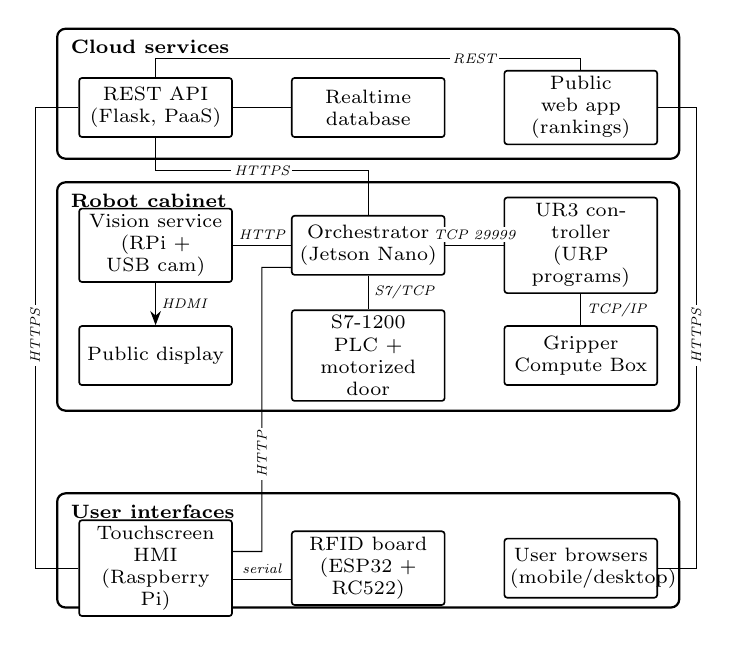
\begin{tikzpicture}[
  mod/.style={draw, semithick, rounded corners=1pt, align=center,
              font=\scriptsize, text width=1.8cm, minimum height=7.5mm,
              inner sep=2pt, fill=white},
  proto/.style={font=\tiny\itshape, fill=white, inner sep=1pt},
  dom/.style={draw, thick, rounded corners=3pt},
  domlbl/.style={font=\scriptsize\bfseries, anchor=north west}
]
% ---- domain boxes
\draw[dom] (0.5,6.15) rectangle (8.4,7.8);
\node[domlbl] at (0.55,7.78) {Cloud services};
\draw[dom] (0.5,2.95) rectangle (8.4,5.85);
\node[domlbl] at (0.55,5.83) {Robot cabinet};
\draw[dom] (0.5,0.45) rectangle (8.4,1.9);
\node[domlbl] at (0.55,1.88) {User interfaces};
% ---- cloud nodes
\node[mod] (api) at (1.75,6.8) {REST API\\(Flask, PaaS)};
\node[mod] (db)  at (4.45,6.8) {Realtime database};
\node[mod] (web) at (7.15,6.8) {Public web app\\(rankings)};
% ---- cabinet nodes
\node[mod] (vis)  at (1.75,5.05) {Vision service\\(RPi + USB cam)};
\node[mod] (orch) at (4.45,5.05) {Orchestrator\\(Jetson Nano)};
\node[mod] (ur3)  at (7.15,5.05) {UR3 controller\\(URP programs)};
\node[mod] (disp) at (1.75,3.65) {Public display};
\node[mod] (plc)  at (4.45,3.65) {S7-1200 PLC +\\motorized door};
\node[mod] (grip) at (7.15,3.65) {Gripper\\Compute Box};
% ---- user interface nodes
\node[mod] (hmi)  at (1.75,0.95) {Touchscreen HMI\\(Raspberry Pi)};
\node[mod] (rfid) at (4.45,0.95) {RFID board\\(ESP32 + RC522)};
\node[mod] (brw)  at (7.15,0.95) {User browsers\\(mobile/desktop)};
% ---- cabinet links
\draw (vis) -- node[proto,above=1pt]{HTTP} (orch);
\draw (orch) -- node[proto,above=1pt]{TCP 29999} (ur3);
\draw (orch) -- node[proto,right=1pt]{S7/TCP} (plc);
\draw[-{Stealth[length=1.8mm]}] (vis) -- node[proto,right=1pt]{HDMI} (disp);
\draw (ur3) -- node[proto,right=1pt]{TCP/IP} (grip);
% ---- user interface links
\draw ([yshift=-4pt]hmi.east) -- node[proto,above=1pt]{serial} ([yshift=-4pt]rfid.west);
\draw ([yshift=6pt]hmi.east) -| (3.1,4.77) -- ([yshift=-8pt]orch.west);
\node[proto, rotate=90] at (3.1,2.4) {HTTP};
\draw (hmi.west) -| (0.22,6.8) -- (api.west);
\node[proto, rotate=90] at (0.22,3.9) {HTTPS};
\draw (brw.east) -| (8.62,6.8) -- (web.east);
\node[proto, rotate=90] at (8.62,3.9) {HTTPS};
% ---- cloud links
\draw (orch.north) -- (4.45,6.0) -- (1.75,6.0) -- (api.south);
\node[proto] at (3.1,6.0) {HTTPS};
\draw (api) -- (db);
\draw (api.north) -- (1.75,7.42) -- (7.15,7.42) -- (web.north);
\node[proto] at (5.8,7.42) {REST};
\end{tikzpicture}
\caption{Logical architecture: the three loosely coupled domains (robot cabinet, cloud services, and user interfaces) and the native protocol used at each interface.}
\label{fig:architecture}
\end{figure}

\subsection{Network Topology and Protocols}
Inside the cabinet, the devices form a star topology around an Ethernet switch with static IPv4 addressing in a private /24 segment; the switch uplinks to the campus network for Internet access. A Jetson Nano single-board computer acts as the edge orchestrator. Instead of imposing a unified middleware, the integration deliberately uses the native protocol of each device: the S7 protocol (through the Snap7 open-source library \cite{b13}) for the PLC, the dashboard server on TCP port 29999 for loading and starting robot programs \cite{b14}, and HTTP/REST for the vision service, the HMI, and the cloud. This choice kept every vendor stack unmodified and reduced the integration surface to a small set of documented calls. Table~\ref{tab:nodes} summarizes the nodes, and Fig.~\ref{fig:topology} shows the resulting topology, including the cloud endpoints.

The alternative of imposing a unified middleware, such as ROS~2 \cite{b16} or an MQTT or OPC~UA integration bus, was considered and discarded: none of the industrial endpoints speaks those protocols natively, so the PLC, the gripper Compute Box, and the robot dashboard would each have required a custom bridge to be written, versioned, and maintained on top of the vendor stack it wraps, adding a layer of indirection without removing any of the underlying protocols. The accepted trade-offs are that the orchestrator is a single point of failure and that coordination is sequential rather than event-driven; scaling to multiple cells or richer telemetry would justify revisiting a message-oriented middleware, but for a single cell with one robot and one PLC, native protocols minimized both the integration effort and the failure surface.

\begin{table}[!t]
\caption{Network Nodes, Roles, and Protocols}
\begin{center}
\footnotesize
\begin{tabular}{|p{2.3cm}|p{2.7cm}|p{2.2cm}|}
\hline
\textbf{Node} & \textbf{Role} & \textbf{Protocols} \\
\hline
Jetson Nano & Edge orchestrator, cycle coordination & HTTP server, S7 client, TCP sockets \\
\hline
Raspberry Pi (vision) & TFLite inference service, public screen media & HTTP (Flask) \\
\hline
Raspberry Pi (HMI) & Touchscreen GUI, RFID bridge & HTTP client, serial \\
\hline
Siemens S7-1200 PLC & Door actuation, interlock logic & S7 over TCP \\
\hline
UR3 robot & Manipulation routines (URP programs) & Dashboard server (TCP 29999) \\
\hline
Gripper Compute Box & Soft gripper control & TCP/IP \\
\hline
Cloud API (PaaS) & REST backend, business logic & HTTPS \\
\hline
Realtime database & Per-user persistence & HTTPS \\
\hline
\end{tabular}
\label{tab:nodes}
\end{center}
\end{table}

\begin{figure}[!t]
\centerline{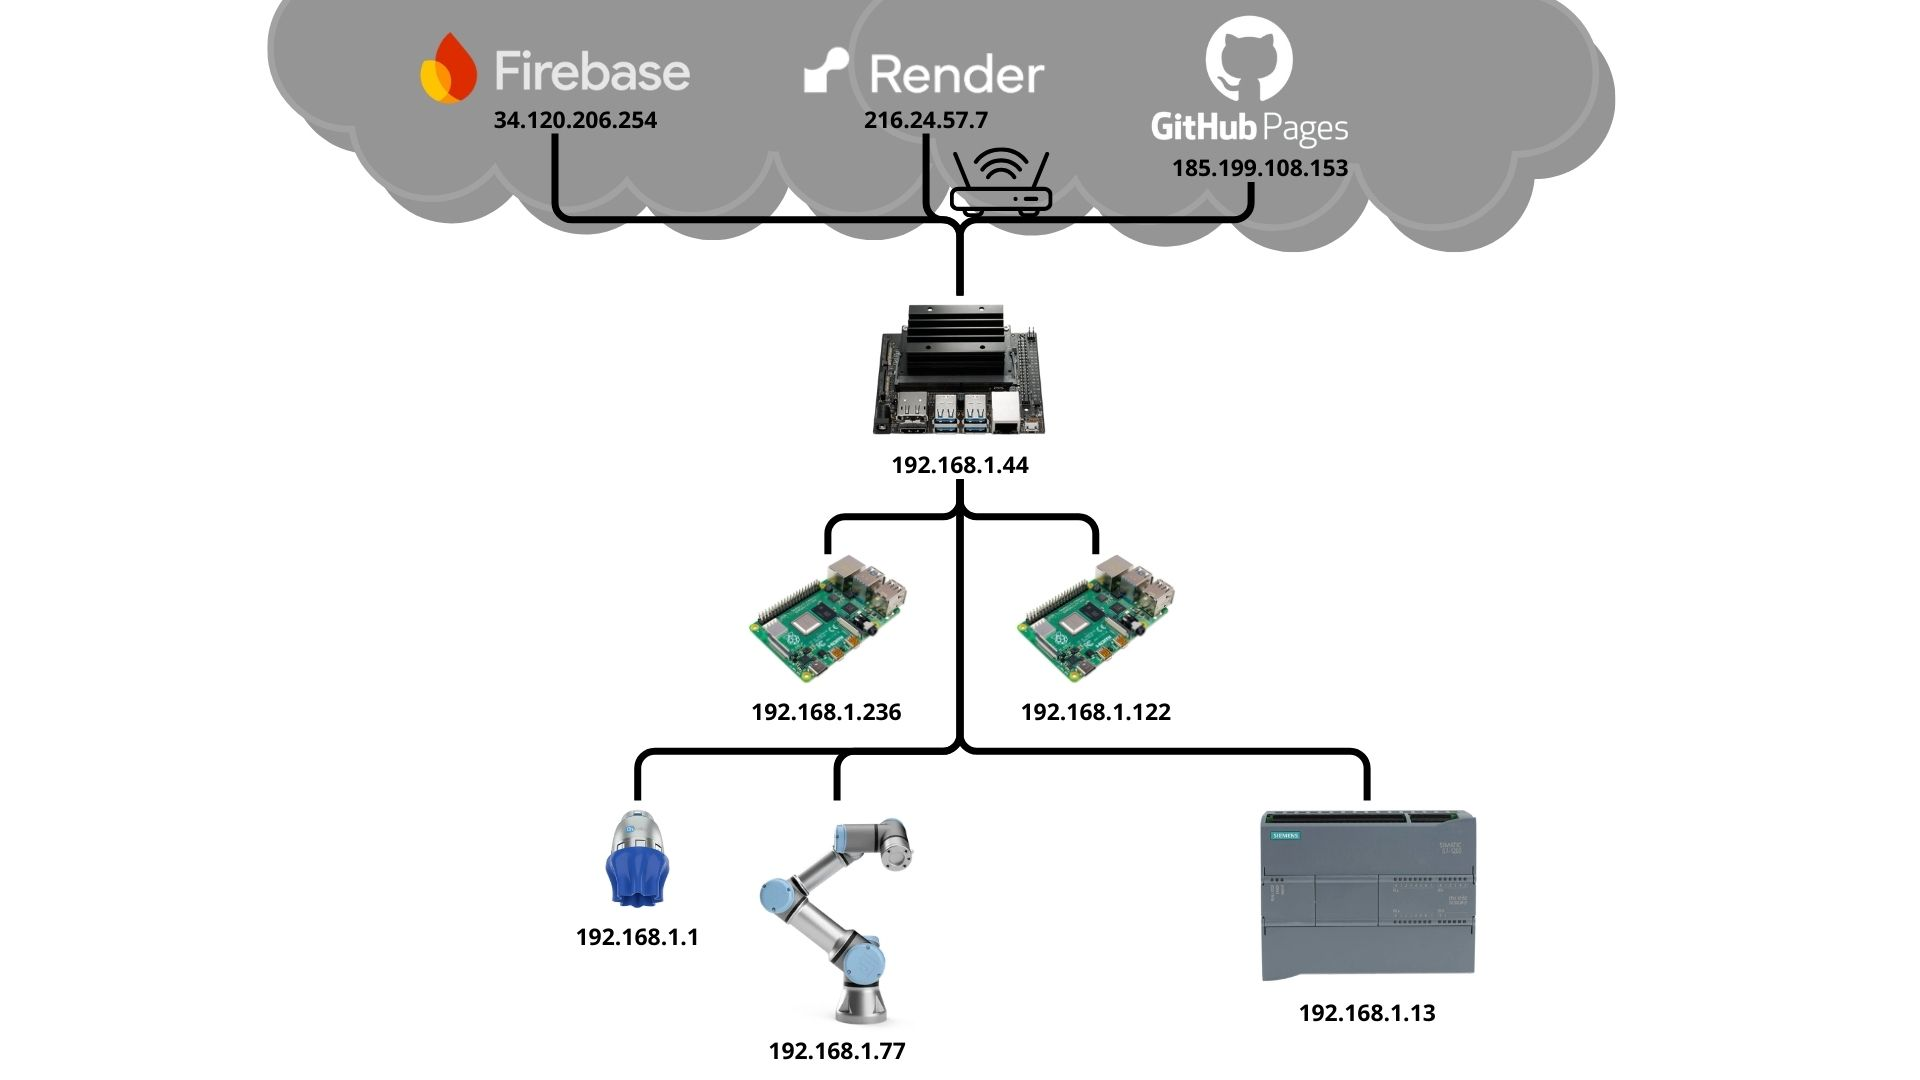
\includegraphics[width=\columnwidth]{Diagrama-topologia.jpg}}
\caption{Network topology: the local star network around the cabinet switch and its links to the cloud services.}
\label{fig:topology}
\end{figure}

\section{Subsystem Design and Integration}
\subsection{Cabinet Structure and Robotic Cell}
The cabinet is built from 40$\times$40~mm aluminum extrusion profiles with a footprint of 1000$\times$920~mm and a height of 2100~mm (Fig.~\ref{fig:prototype}). The UR3 is mounted at the top of the frame, centered along the width, so that its workspace covers both the reception tray and the classification containers. Three bins are placed at the rear of the structure on a reinforced shelf; profiles at 45$^{\circ}$ and two caster-terminated legs stiffen the frame against the cantilevered loads. A 50-inch display above the bins shows public feedback during operation. The front of the cabinet is enclosed with 3-mm acrylic and PVC panels, separating users from the robot workspace; combined with the bounded forces of the collaborative arm \cite{b10}, \cite{b11}, this provides two independent layers of protection.

\begin{figure}[!t]
\centerline{\includegraphics[width=0.8\columnwidth]{Gabinete_robot.jpg}}
\caption{Integrated prototype: aluminum frame, UR3 robot with soft gripper, reception door, classification bins, public display, and HMI.}
\label{fig:prototype}
\end{figure}

For manipulation, the UR3 carries an OnRobot SG soft gripper, whose elastomer membrane adapts to variable geometries and fragile surfaces such as glass bottles. The gripper is managed by its Compute Box, connected to the cabinet switch over Ethernet and exposed to the robot controller as scriptable commands; grasping and releasing are performed by commanding target widths (e.g., \texttt{sg\_grip(30,...)} to grasp and \texttt{sg\_grip(75,...)} to release).

All trajectories are encapsulated as URP programs stored in the robot controller: an observation routine that places the camera viewpoint over the reception tray, one collection routine per material class, and one deposit routine per container. The orchestrator never commands joint motions directly during normal operation; it only selects which program to load and play. This decoupling keeps the kinematics where they are best maintained (the teach pendant) and the decision logic where it is best versioned (the orchestrator code).

\subsection{Waste Reception Module}
Objects enter the cabinet through a 170$\times$330~mm aperture closed by a horizontally sliding door. The door runs on V-slot wheels and is driven by a belt-pulley transmission coupled to a NEMA~17 stepper motor. A microstepping driver (9--42~V) is configured for 200 pulses per revolution and a phase current of 1.5--1.7~A. A Siemens S7-1200 PLC generates the pulse and direction trains from a ladder program; the driver inputs PUL+ and DIR+ are tied to +24~V, while PUL$-$ and DIR$-$ are switched by PLC outputs Q0.0 and Q0.1. The orchestrator commands the door by writing two memory bits (open and close) over the S7 protocol and reading them back to confirm the state.

Safety is implemented as a hardwired chain that is independent of all software: a normally closed emergency stop and a normally closed stop button feed a normally open start button that energizes an industrial relay with a self-holding auxiliary contact. The relay contacts switch both the 120~VAC feed of the robot and gripper and the 24~VDC supply of the stepper driver, so pressing the emergency stop removes power from every actuator regardless of the state of the PLC, the orchestrator, or the network. Control logic (24~VDC) and power loads are kept on separate circuits throughout the panel.

\subsection{Embedded Vision and Classification}
A USB camera observes the reception tray from the viewpoint defined by the robot observation pose, and is attached to a dedicated Raspberry Pi that runs the classification service. The classifier was obtained by transfer learning with Teachable Machine \cite{b8}, which fine-tunes a MobileNet-family backbone \cite{b7}, and was exported to TensorFlow Lite \cite{b9} for embedded inference. Four classes are distinguished: glass, can, Tetra Pak, and a background class (``bg'') that captures empty scenes and non-target objects. Table~\ref{tab:dataset} summarizes the training dataset, which was captured against a dark background under controlled illumination, varying object pose, color, and wear (Fig.~\ref{fig:training}).

\begin{table}[!t]
\caption{Training Dataset Composition}
\begin{center}
\begin{tabular}{|l|c|l|}
\hline
\textbf{Class} & \textbf{Images} & \textbf{Variability captured} \\
\hline
Glass & 49 & Orientations of transparent bottles \\
\hline
Can & 83 & Colors, frontal/lateral/top views \\
\hline
Tetra Pak & 79 & Fill levels and wear \\
\hline
Background & 10 & Empty tray, irrelevant objects \\
\hline
\end{tabular}
\label{tab:dataset}
\end{center}
\end{table}

\begin{figure}[!t]
\centerline{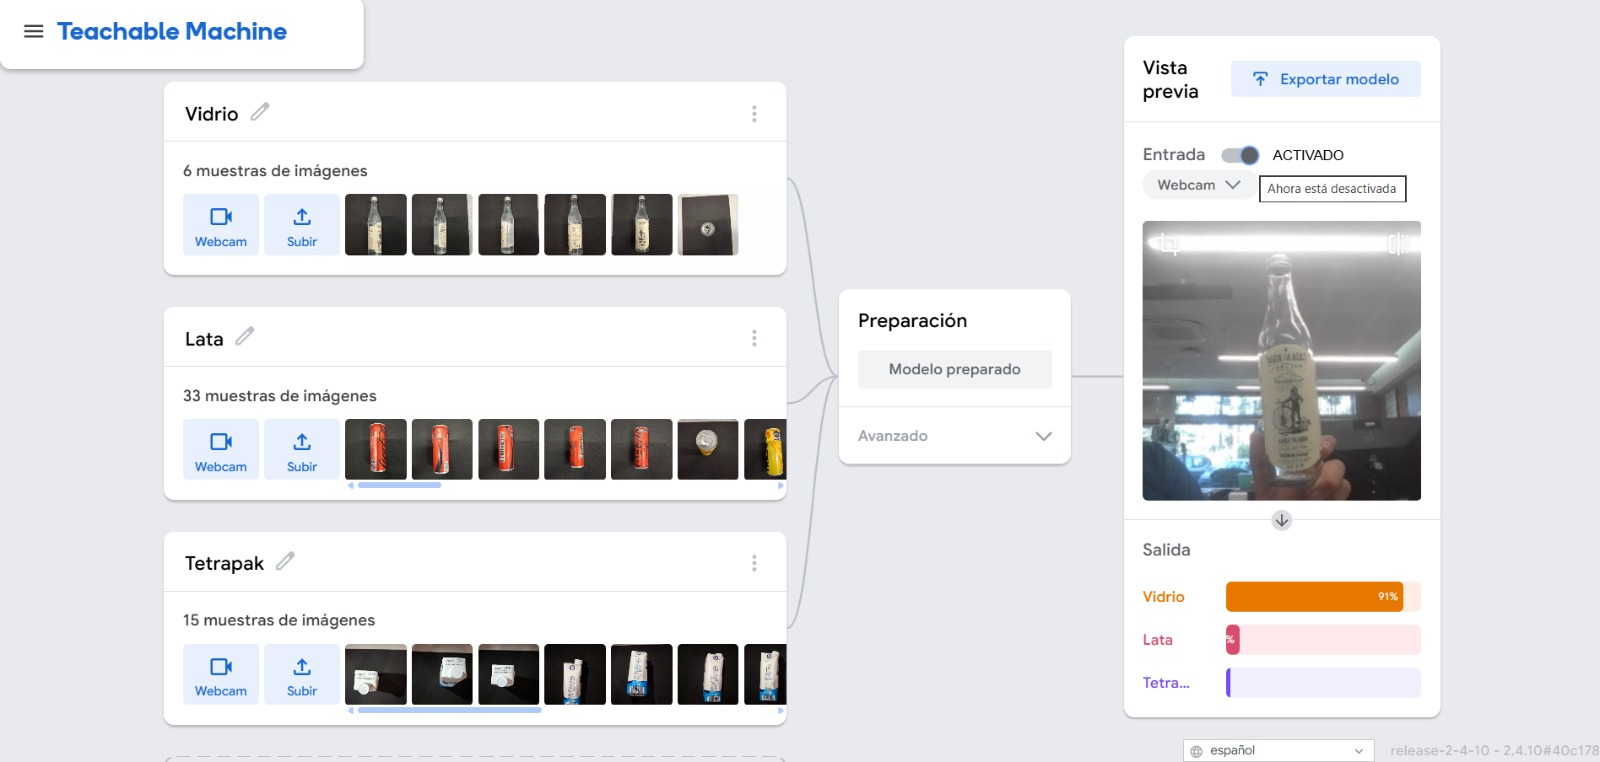
\includegraphics[width=\columnwidth]{Entrenamiento.png}}
\caption{Training of the four-class waste classifier by transfer learning and its real-time validation with the system camera.}
\label{fig:training}
\end{figure}

The service exposes an HTTP endpoint (\texttt{/identify}) that returns the detected label as JSON. To reduce the effect of transient misclassifications, the reported label is the statistical mode of several consecutive predictions taken within a capture window, rather than a single frame decision. When the result is ``bg'', the orchestrator aborts the cycle and returns the robot to its home pose, which prevents spurious manipulation of invalid objects.

\subsection{User Identification and Local HMI}
User identification is handled by a custom single-layer PCB designed around an ESP32-WROOM-32 module and an RC522 13.56-MHz RFID reader connected over SPI (Fig.~\ref{fig:pcb}). The board includes a buzzer for audible confirmation, two status LEDs, a user switch, and a 4-pin UART header for programming and debugging. Design rules followed embedded RF practice: a copper and fastener keep-out region under the ESP32 antenna, short parallel SPI traces, and 1206 passive footprints for manual rework. The board was fabricated professionally and assembled and tested in the laboratory.

\begin{figure}[!t]
\centerline{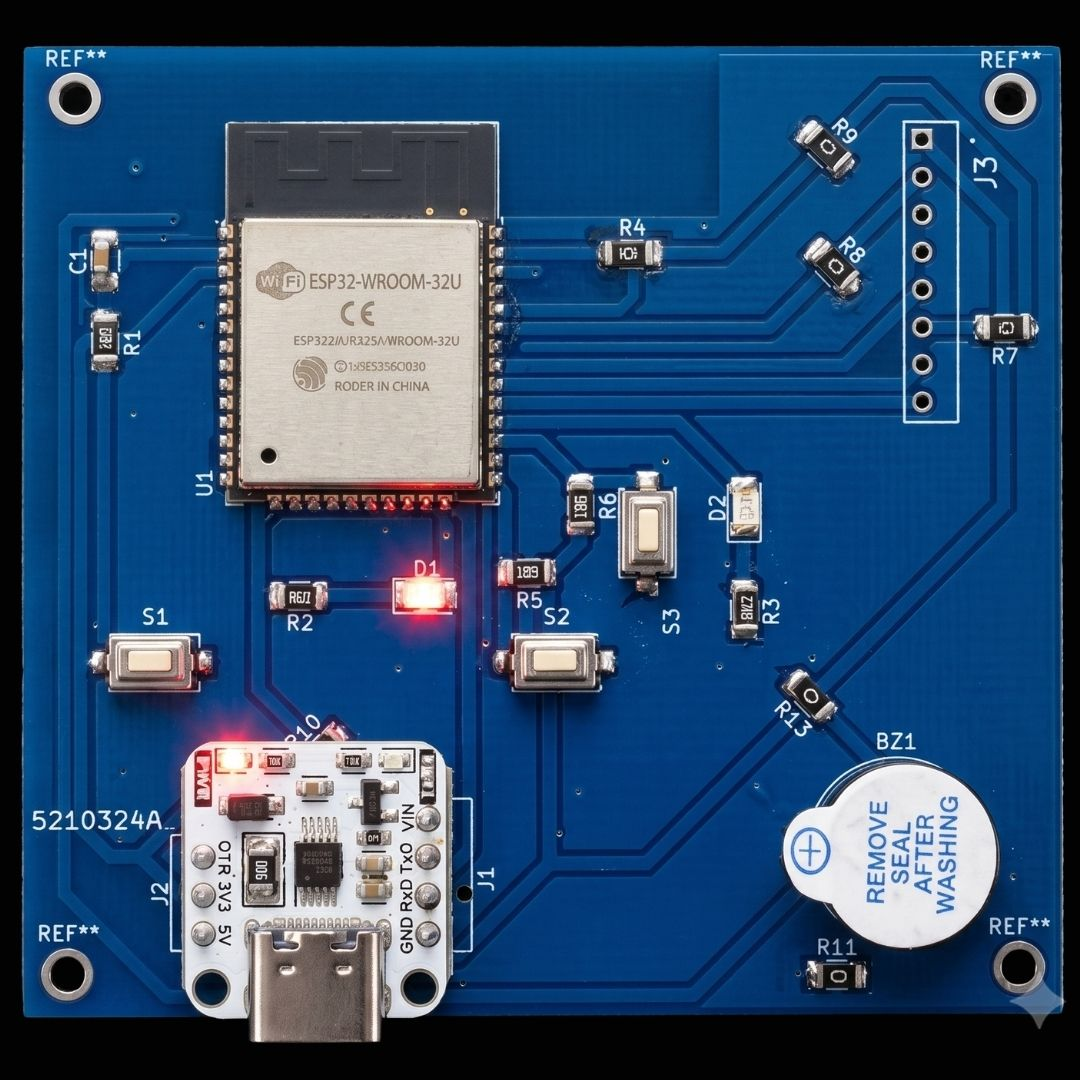
\includegraphics[width=0.75\columnwidth]{PCB-real.jpg}}
\caption{Custom RFID identification board: ESP32-WROOM-32, RC522 reader over SPI, buzzer, status LEDs, and UART programming header.}
\label{fig:pcb}
\end{figure}

The local HMI runs on a Raspberry Pi with a 7-inch touchscreen, mounted on the cabinet at $-45^{\circ}$ using printed PLA and laser-cut acrylic parts for comfortable interaction (Fig.~\ref{fig:hmi}). The graphical application, developed in Tkinter, implements three flows: (i) \emph{login}, where scanning a card retrieves the user name and accumulated score; (ii) \emph{account creation}, where a new card identifier is associated with a name and pushed to the backend as JSON over HTTP; and (iii) \emph{anonymous recycling}, which allows participation without scoring. After a successful login, the user triggers the classification cycle from the screen, and the interface reports progress, errors, and the points obtained.

\begin{figure}[!t]
\centerline{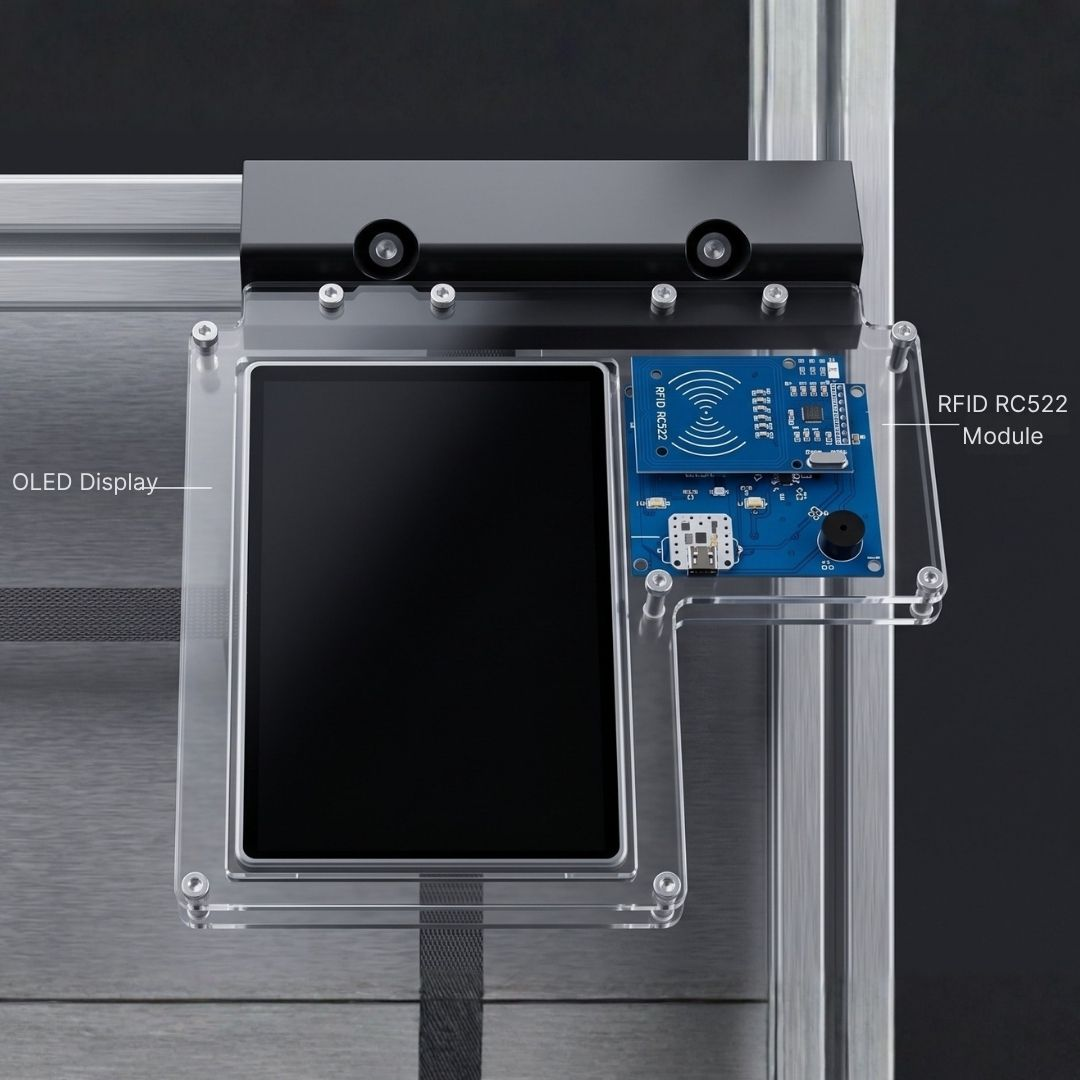
\includegraphics[width=0.8\columnwidth]{UI.jpg}}
\caption{Local HMI: 7-inch touchscreen and RFID reading zone mounted on the cabinet front.}
\label{fig:hmi}
\end{figure}

\subsection{Edge Orchestration}
The Jetson Nano runs a Flask server and an event-driven main loop that coordinate the complete cycle. The HMI signals the start of a deposit through a \texttt{/empezarObjeto} request and binds the active user session through \texttt{/consulta}. When the start event arrives, the orchestrator executes the following sequence:
\begin{enumerate}
\item send the UR3 to its home pose;
\item command the PLC to open the door (timed motion followed by an explicit stop command);
\item load and play the observation routine on the robot;
\item query the vision service and obtain the windowed classification;
\item close the door;
\item if the label is a valid material, load and play the corresponding collection and deposit routines through the dashboard interface; and
\item when both a user session and a completed routine have been registered, post the point increment to the cloud API and return to home.
\end{enumerate}
Every stage is guarded with timeouts and exception handling, so a failure in any link (robot telemetry loss, vision timeout, PLC disconnection) degrades to a safe abort that closes the door and returns the robot to home. While idle, the orchestrator pushes promotional media to the public display every 17~s through the vision node, and during collection it streams the robot point of view to the same screen, reinforcing user engagement.

\subsection{Cloud Services and Traceability}
The backend is a Flask REST API deployed on a platform-as-a-service provider, with credentials injected through environment variables and permissive CORS so that heterogeneous clients (robot, HMI, web) can reach it. Persistence uses a managed real-time database \cite{b15} with a simple per-user schema: name, creation date, and one counter per material (\texttt{lata}, \texttt{vidrio}, \texttt{tetra}). The API exposes endpoints to create users, query a profile, increment a counter for a validated deposit, and retrieve top-100 rankings by total and by material, with input validation and explicit error responses for unknown users or invalid categories.

A public single-page web application consumes these endpoints and presents each participant with their accumulated counts and position in the rankings, on a responsive layout for mobile and desktop. In the intended flow, every increment originates from a physically completed robot cycle, so the database constitutes a traceable record that links users, materials, and timestamps; the rankings convert that record into a gamification incentive \cite{b12}.

\section{Functional Validation and Discussion}
\subsection{Link-Level Integration Tests}
Integration followed a bottom-up strategy in which every interface was validated in isolation with short test scripts before composing the full cycle: writing and reading back the PLC door bits over S7; commanding UR3 joint motions with a 0.02-rad arrival tolerance and telemetry-loss guards; loading and starting URP programs through the dashboard server; and requesting classifications over HTTP. These tests located configuration faults (addressing, program paths, timeouts) early, when they were cheap to fix, and produced a small regression suite that remained useful during the final assembly.

\subsection{End-to-End Operation}
The integrated prototype executed complete cycles on real waste items of the three target fractions during laboratory demonstration sessions: a user authenticates with an RFID card, deposits an object through the motorized door, the robot observes and the embedded classifier labels the item, the UR3 collects it with the soft gripper and deposits it in the corresponding bin, and the cloud counters update immediately, becoming visible in the public rankings at the end of the cycle.

Qualitatively, the classifier behaved as expected from its training data: glass bottles were recognized most reliably, aided by their distinctive silhouette and brightness; cans were classified correctly across different colors and orientations; Tetra Pak containers were correct in most attempts; and the background class rejected empty scenes and non-target objects, preventing spurious robot motion. The windowed-mode decision visibly reduced label flickering compared to single-frame queries. The hardwired safety chain was exercised during the sessions, and pressing the emergency stop removed power from the robot, gripper, and door driver as designed.

\subsection{Discussion and Limitations}
The clearest benefit of the architecture was the degree of independence between modules. Because each subsystem hides behind a narrow interface, the vision model can be retrained and redeployed without touching robot routines, deposit trajectories can be re-taught on the pendant without rebuilding the orchestrator, and the cloud schema evolved during development without affecting the cabinet. The subsystems were in fact developed in parallel by different team members and integrated late with limited rework, which we attribute to the protocol-level decoupling described in Section~III.

The current prototype also has clear limitations. The training dataset is small (221 images) and was captured under controlled illumination, so robustness to lighting changes and unseen packaging variants is limited. The validation reported here is functional and qualitative: a statistically rigorous campaign measuring per-class accuracy, confusion patterns, and cycle times remains to be carried out. The cycle assumes a single object per deposit and uses fixed grasp poses, so items must rest in an expected region of the tray. Finally, the system depends on network availability, and the free-tier cloud deployment introduces cold-start latency on the first request. Moreover, with permissive CORS and no origin authentication on the increment endpoint, the cloud record is trustworthy only within the intended flow; securing the robot-to-cloud channel with per-device credentials remains pending work.

\section{Conclusions and Future Work}
This paper presented the design and integration of a modular cyber-physical system that automates the classification of glass, cans, and Tetra Pak containers using a collaborative robot, embedded vision, industrial door control, RFID user identification, and cloud traceability with gamified feedback. The three-domain architecture and the use of native device protocols kept the integration surface small and allowed parallel development of subsystems that were later composed into complete, automatically chained operation cycles on real waste items.

Future work will proceed along four lines: enlarging and diversifying the training dataset and evaluating the classifier with formal metrics under uncontrolled illumination; instrumenting the orchestrator to log cycle times and outcomes for a quantitative performance campaign; adding object pose estimation to relax the fixed-grasp assumption; and extending the material set and the gamification mechanics (e.g., rewards and campaigns) supported by the cloud layer.

% Acknowledgment intentionally omitted in the double-blind version.
%\section*{Acknowledgment}
%(Add funding and institutional acknowledgments in the camera-ready version.)

\begin{thebibliography}{00}
\bibitem{b1} S. Kaza, L. Yao, P. Bhada-Tata, and F. Van Woerden, \emph{What a Waste 2.0: A Global Snapshot of Solid Waste Management to 2050}. Washington, DC, USA: World Bank, 2018.
\bibitem{b2} E. A. Lee, ``Cyber physical systems: Design challenges,'' in \emph{Proc. 11th IEEE Int. Symp. Object and Component-Oriented Real-Time Distributed Computing (ISORC)}, Orlando, FL, USA, 2008, pp. 363--369.
\bibitem{b3} L. Monostori \emph{et al.}, ``Cyber-physical systems in manufacturing,'' \emph{CIRP Annals}, vol. 65, no. 2, pp. 621--641, 2016.
\bibitem{b4} T. J. Lukka, T. Tossavainen, J. V. Kujala, and T. Raiko, ``ZenRobotics Recycler -- Robotic sorting using machine learning,'' in \emph{Proc. Int. Conf. Sensor-Based Sorting (SBS)}, Aachen, Germany, 2014.
\bibitem{b5} M. Yang and G. Thung, ``Classification of trash for recyclability status,'' CS229 Project Report, Stanford University, Stanford, CA, USA, 2016.
\bibitem{b6} O. Adedeji and Z. Wang, ``Intelligent waste classification system using deep learning convolutional neural network,'' \emph{Procedia Manufacturing}, vol. 35, pp. 607--612, 2019.
\bibitem{b7} M. Sandler, A. Howard, M. Zhu, A. Zhmoginov, and L.-C. Chen, ``MobileNetV2: Inverted residuals and linear bottlenecks,'' in \emph{Proc. IEEE/CVF Conf. Computer Vision and Pattern Recognition (CVPR)}, Salt Lake City, UT, USA, 2018, pp. 4510--4520.
\bibitem{b8} M. Carney \emph{et al.}, ``Teachable Machine: Approachable web-based tool for exploring machine learning classification,'' in \emph{Extended Abstracts CHI Conf. Human Factors in Computing Systems}, Honolulu, HI, USA, 2020, pp. 1--8.
\bibitem{b9} M. Abadi \emph{et al.}, ``TensorFlow: A system for large-scale machine learning,'' in \emph{Proc. 12th USENIX Symp. Operating Systems Design and Implementation (OSDI)}, Savannah, GA, USA, 2016, pp. 265--283.
\bibitem{b10} J. E. Colgate, W. Wannasuphoprasit, and M. A. Peshkin, ``Cobots: Robots for collaboration with human operators,'' in \emph{Proc. ASME Int. Mechanical Engineering Congress and Exposition}, Atlanta, GA, USA, 1996, pp. 433--439.
\bibitem{b11} \emph{Robots and Robotic Devices -- Collaborative Robots}, ISO/TS 15066:2016, International Organization for Standardization, Geneva, Switzerland, 2016.
\bibitem{b12} S. Deterding, D. Dixon, R. Khaled, and L. Nacke, ``From game design elements to gamefulness: Defining `gamification','' in \emph{Proc. 15th Int. Academic MindTrek Conf.}, Tampere, Finland, 2011, pp. 9--15.
\bibitem{b13} D. Nardella, ``Snap7: Step7 Ethernet communication suite,'' 2013. [Online]. Available: https://snap7.sourceforge.net
\bibitem{b14} Universal Robots A/S, ``Dashboard server -- CB-Series and e-Series interface,'' Odense, Denmark. [Online]. Available: https://www.universal-robots.com/articles/ur/dashboard-server-cb-series-port-29999/
\bibitem{b15} Google LLC, ``Firebase Realtime Database documentation.'' [Online]. Available: https://firebase.google.com/docs/database
\bibitem{b16} S. Macenski, T. Foote, B. Gerkey, C. Lalancette, and W. Woodall, ``Robot Operating System 2: Design, architecture, and uses in the wild,'' \emph{Science Robotics}, vol. 7, no. 66, eabm6074, 2022.
\end{thebibliography}

\end{document}
